\chapter{Design}
\textbf{Versionshistorik}
\begin{longtabu} to \linewidth{@{}l l l X[j]@{}}
    Version &    Dato &    Ansvarlig &    Beskrivelse\\[-1ex]
    \midrule
    1.0		&	20-10-2015 &	 Alle	& Første udkast til domænemodel, bdd, ibd og sekvensdiagrammer	\\[-1ex]
    1.1		&	21-10-2015	&	Alle	& Små ændringer i bdd og ibd efter møde med vejleder \\[-1ex]
    1.2		&	27-10-2015	&	Alle	& Ændring af bdd og ibd efter møde med Kim; blokkene filter og forstærker er blevet lagt sammen under blokken instrumenteringsforstærker\\[-1ex]
    1.3  	&	02-11-2015	&	Alle	& Begyndte at oprette Design-dokumentet. Udkast til klassediagrammer for UC \\[-1ex]
    1.4		&	04-11-2015	&	Alle	& Skrevet hardward design afsnittet. Små rettelser i de andre afsnit i design, så det er klar til review \\[-1ex]
\label{version_Systemark}
\end{longtabu}

\section{Systemarkitektur} 
Igennem BBD og IBD vil det overordnede blodtryksmålersystem beskrives i forhold til hvilke blokke systemet består af, og hvordan de interagerer med hinanden. 

\subsection{BBD-diagram}
På figur 2.1 ses BDD-diagrammet for systemet. BBD viser de forskellige blokke for systemet og hvilke porte de består af. I tabel 2.2 ses en beskrivelse af blokkene. 

\begin{figure}[H]
	\centering
	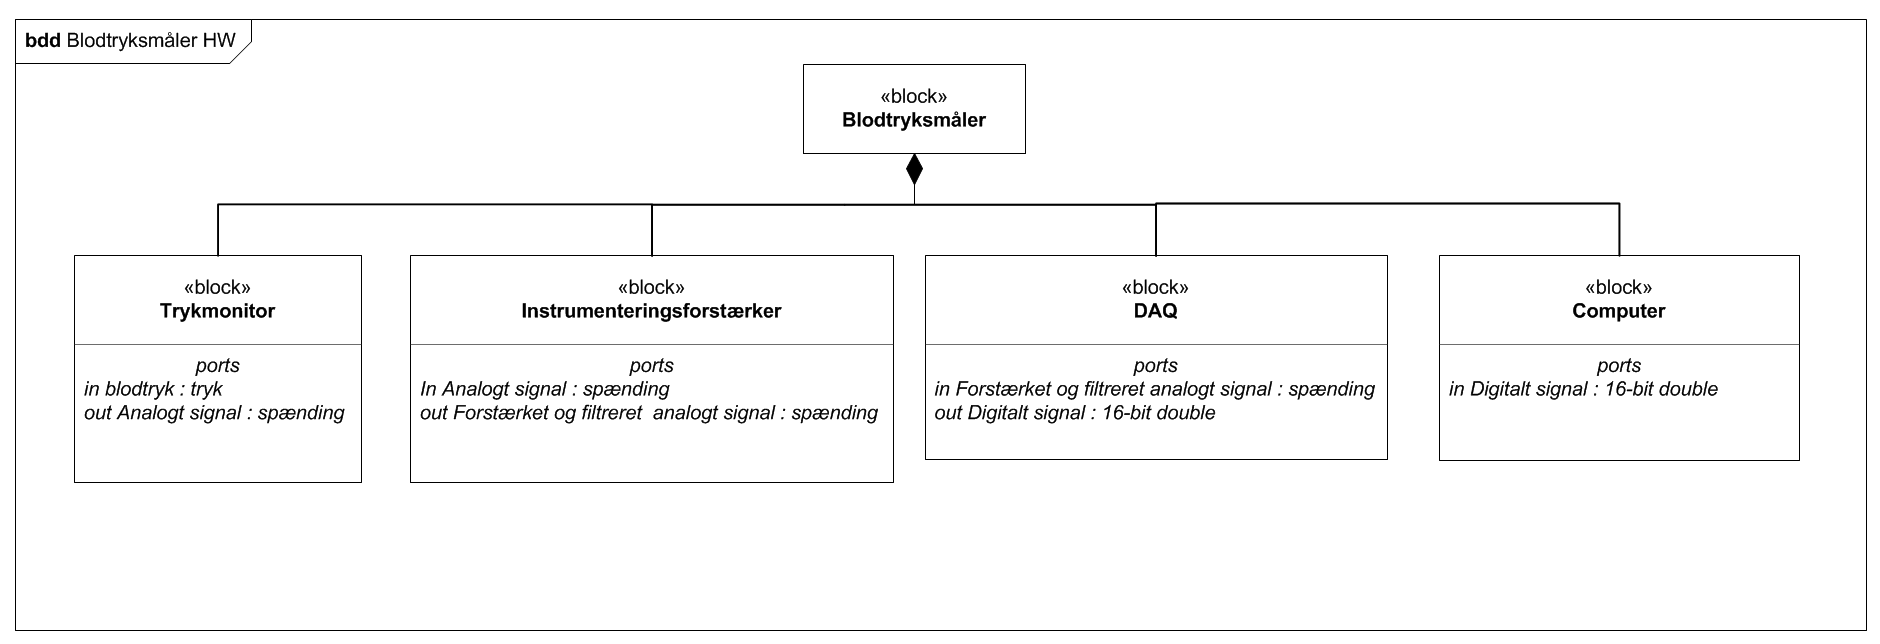
\includegraphics[width=1\textwidth]{Figurer/Snip20151104_45}
	\caption{BBD-diagram}
	\label{fig:BBD-diagram}
\end{figure}

\begin{longtabu} to \linewidth{@{}l X[j]@{}}
	\textbf{Blok} &	\textbf{Beskrivelse} \\[-1ex]
	\midrule
	Blodtryksmåler & Det overordnede system, som indeholder Trykmonitor, Instrumenteringsforstærker, DAQ og Computer\\[-1ex]
	Trykmonitor & Registrerer en fysisk størrelse i form af en trykændring. I dette system anvendes en transducer. Transduceren har til opgave at transformere den fysiske størrelse til en elektrisk spænding, som viderebehandles gennem de resterne hardware blokke  \\[-1ex]
	Instrumenteringsforstærker & Består af to dele. En forstærker-del og en filterings-del. Det analoge signal fra Trykmonitoren bliver via denne blok forstærket og filteret\\[-1ex]
	DAQ & Konverterer det analoge signal fra Trykmonitoren til et digitalt signal\\[-1ex]
	Computer & Indeholder software til systemet, som er kodet i Visual Studio C\#. Softwaren kan blandt andet vise det digitale signal grafisk. Softwaren kan ligeledes kalibrere, nulpunktsjustere og gemme målinger samt aktivere og deaktiver filter\\[-1ex]
	\caption{Beskrivelse af blokkene for systemet}
	\end{longtabu}
	
\subsection{IBD-diagram}
På figur 2.2 ses IBD-diagrammet for systemet. IBD viser, hvordan de forskellige blokke intergerer med hinanden. IBD fortæller signalets behandling gennem systemet - altså hvordan signalet transformeres fra et målt fysisk tryk til et digitalt signal, som softwaren kan videre behandle og vise grafisk. 

\begin{figure}[H]
	\centering
	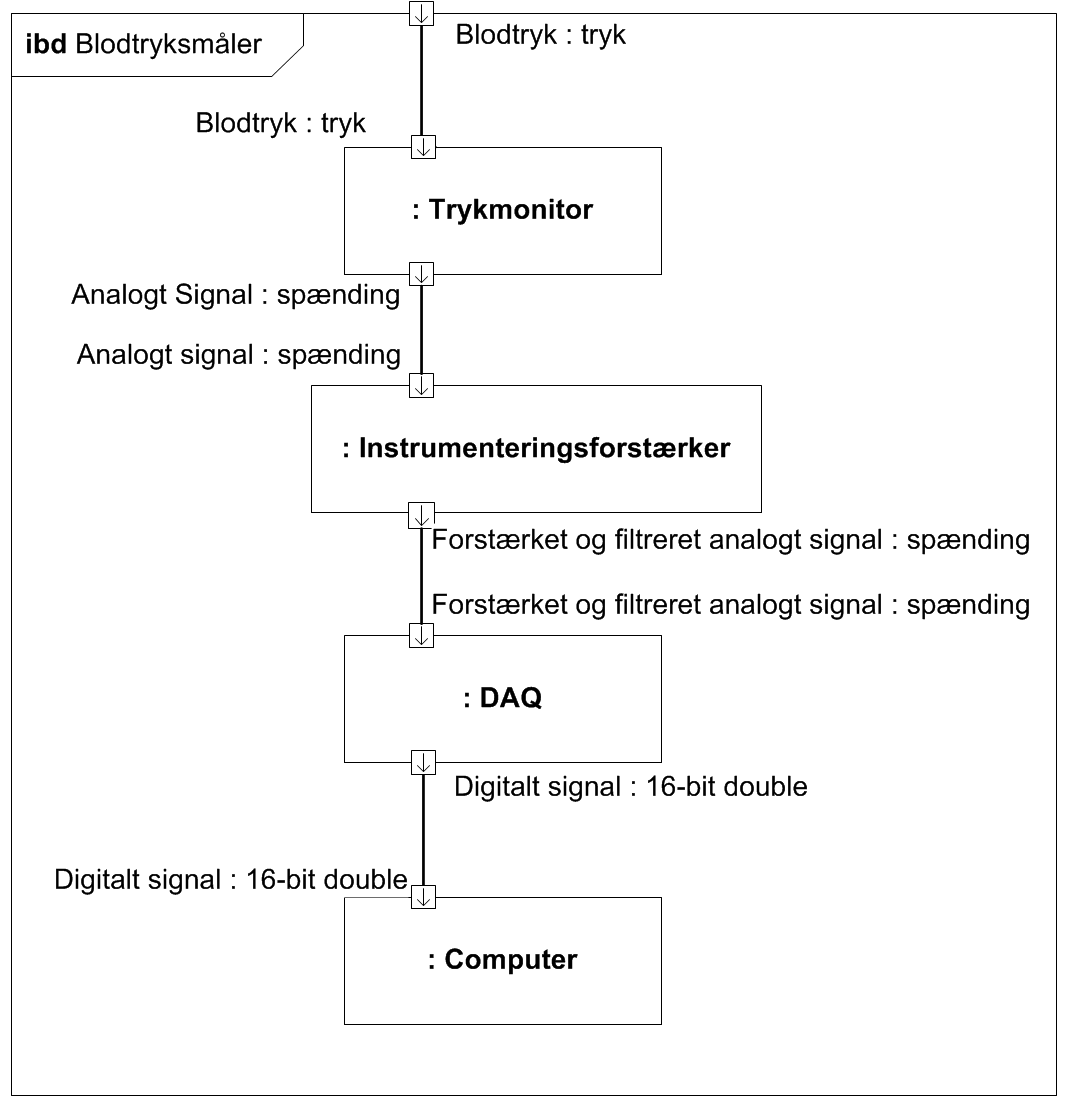
\includegraphics[width=0.8\textwidth]{Figurer/Snip20151102_7}
	\caption{IBD-diagram}
	\label{fig:IBD-diagram}
\end{figure}

\section{Grænseflader}
Kommunikationsprotokol for hardware blokkene ses i tabel 2.3. Det er en beskrivelse og specifikation af hvilken indgang- og udgangssignal de forskellige blokke har.   

\begin{longtabu} to \linewidth{@{}l l l l X[j]@{}}
	\textbf{Grænseflade} & \textbf{Signal} & \textbf{Type} & \textbf{Format} & \textbf{Værdi} \\[-1ex]
	\midrule
	Trykmoniter & Blodtryk & in & Tryk & 0 - 300 mmHg \\[-1ex]
				& Analogt & out & Spænding & +/- 13,5mV \\[-1ex]
	Forstærker  & Analogt & in & Spænding & +/- 13,5mV \\[-1ex]
				& Forstærket analogt & out & Spænding & +/- 5V \\[-1ex]
	Filter 		& Forstærket analogt & in & Spænding & +/- 5V \\				[-1ex]
				& Filteret analogt & out & Spænding & +/- 5V \\[-1ex]
	DAQ			& Filteret analogt & in & Spænding & +/- 5V \\				[-1ex]	
				& Digitalt & out & 16-bit double & +/- 5 \\[-1ex]
	Computer	& Digitalt & in & 16-bit double & +/- 5 \\[-1ex]
	\caption{Kommunikationsprotokol}	
\end{longtabu}


\section{Hardware arkitektur}
Herunder er de krævede specifikationer for hardwaren beskrevet. 
 
\subsection{bdd}

\begin{figure}[H]
	\centering
	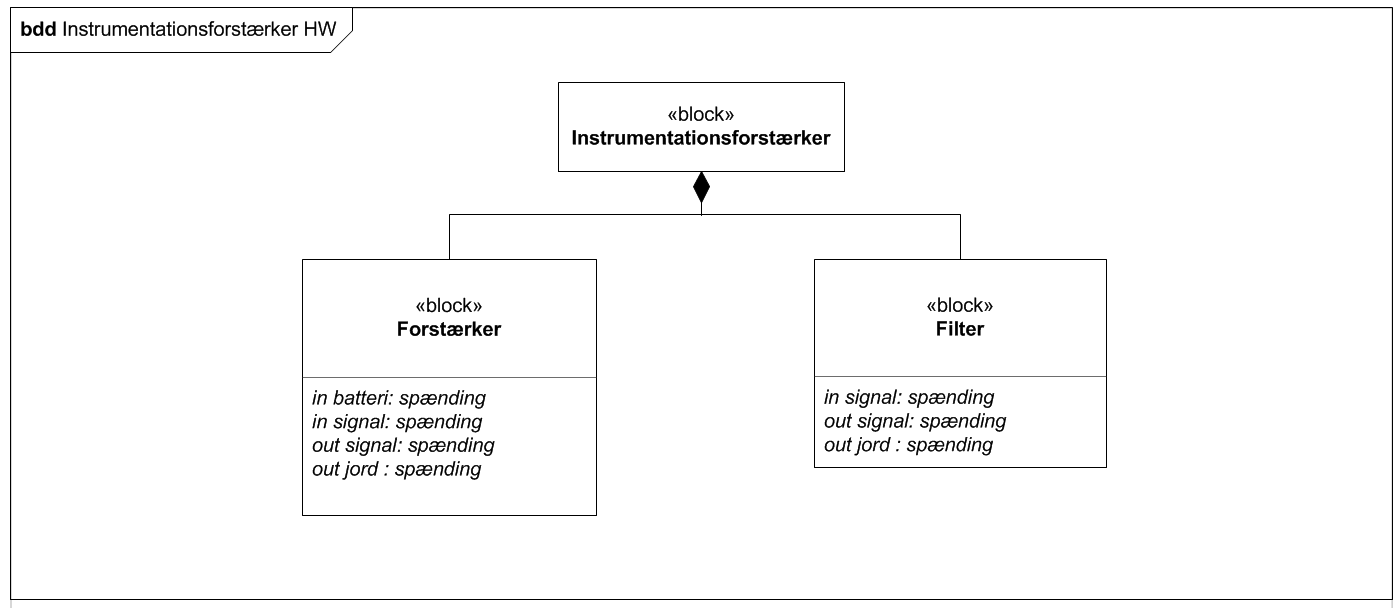
\includegraphics[width=1\textwidth]{Figurer/Snip20151104_46}
	\caption{bdd-diagram for Instrumenteringsforstærker HW}
	\label{fig:bddhw-diagram}
\end{figure}

\subsection{ibd}

\begin{figure}[H]
	\centering
	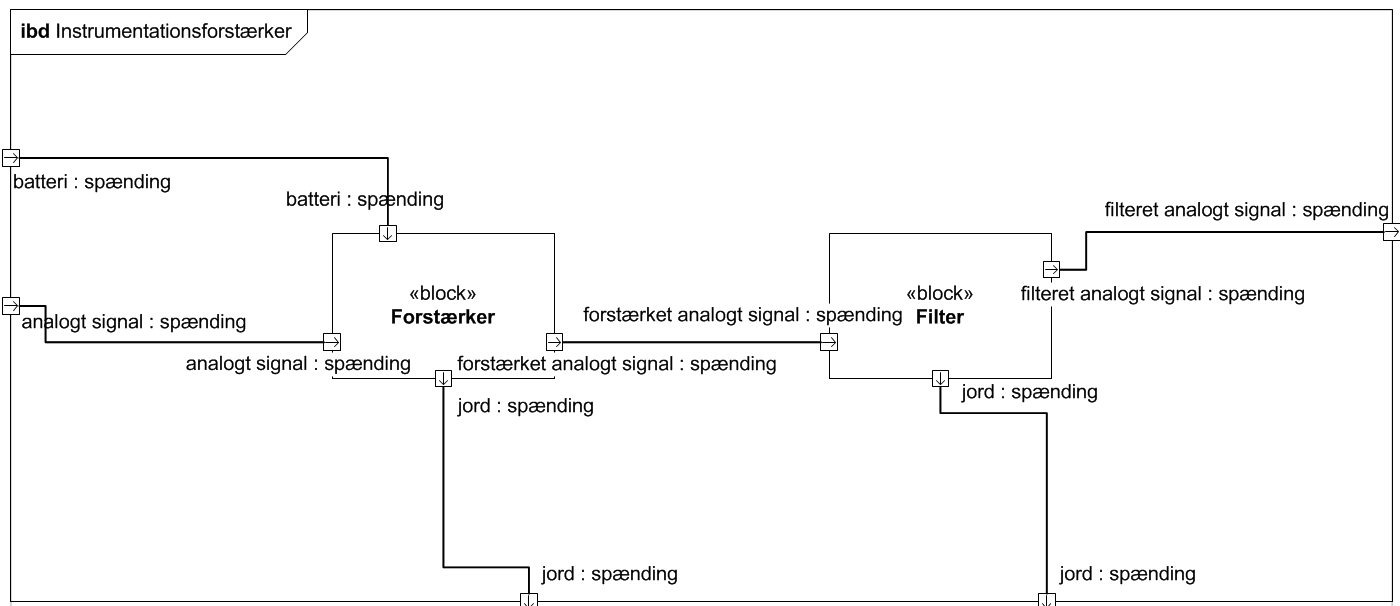
\includegraphics[width=1\textwidth]{Figurer/Snip20151104_48}
	\caption{ibd-diagram for Instrumenteringsforstærker HW}
	\label{fig:ibdhw-diagram}
\end{figure}

\subsection{Grænseflader}

\begin{longtabu} to \linewidth{@{}l l l l X[j]@{}}
	\textbf{Grænseflade} & \textbf{Signal} & \textbf{Type} & \textbf{Format} & \textbf{Værdi} \\[-1ex]
	\midrule
	Forstærker & Batteri & in & Spænding & +/- 9V \\[-1ex]
			   & Analogt & in & Spænding & +/- 13,5mV \\[-1ex]
			   & Jord	 & out & Spænding & 0V \\[-1ex]
			   & Forstærket analogt & out & Spænding & +/- 5V \\[-1ex]
	Filter	   & Forstærket analogt & in & Spænding & +/- 5V\\[-1ex]
			   & Jord	 & out & Spænding & +/- 5V\\[-1ex]
			   & Filteret analogt & out & Spænding & +/- 5V\\[-1ex]
	\caption{Kommunikationsprotokol for Instrumenteringsforstærke}	
\end{longtabu}

\subsection{Tryktransducer}
\subsubsection{Specifikationer}
\begin{itemize}
	\item Måleprobe kan indsættes intravenøst
	\item Operationel trykinterval 0-300 mmHg
	\item Udgangssignal: 2 udgange; +/- udgang
	\item Sensitivitet: 5$\mu$/V/V/mmHg 
	\item Operationstemperatur: 15-40 grader Celcius
\end{itemize}

 \subsection{Instrumentationsforstærker}
 
 
 \subsubsection{Filterblok}
 \subsubsection{Specifikationer}
 \begin{itemize}
 	\item 2. Ordens lavpasfilter
 	\item Cutofffrekvens: 50 Hz
 	\item Unity gain (ingen forstærkning)
 	\item -20 dB ved 500 Hz
 	\item Infinite indgangsimpedans
 	\item Indgangsspænding +/- 5 V
 	\item Eksitationsspænding +/- 9 V
 \end{itemize}
 
  
 
 \subsubsection{Forstærkerblok}
 \subsubsection{Specifikationer}
 \begin{itemize}
 	\item Gain: 370
 	\item Indgangspænding: +/- 0-14 mV
 	\item Eksitationsspænding: +/- 9V
 	\item Outputspænding: +/- 5 V
 	\item Båndbredde: 100 Hz
 \end{itemize}

\section{Software arkitektur}

\subsection{Domænemodel}
Domænemodellen er skabt på baggrund af de seks Use Cases og fungerer som et middel til at skabe et samlet overblik over systemet. Gennem navneordsanalyse er de konceptuelle klasser fundet. I modellen beskrives, hvordan de konceptuelle klasser og aktører interagerer med hinanden. Controlleren er ikke en konceptuel klasse, men det er den, der sørger for at systemet fungerer optimalt, og udfører kommandoer.

\begin{figure}[H]
	\centering
	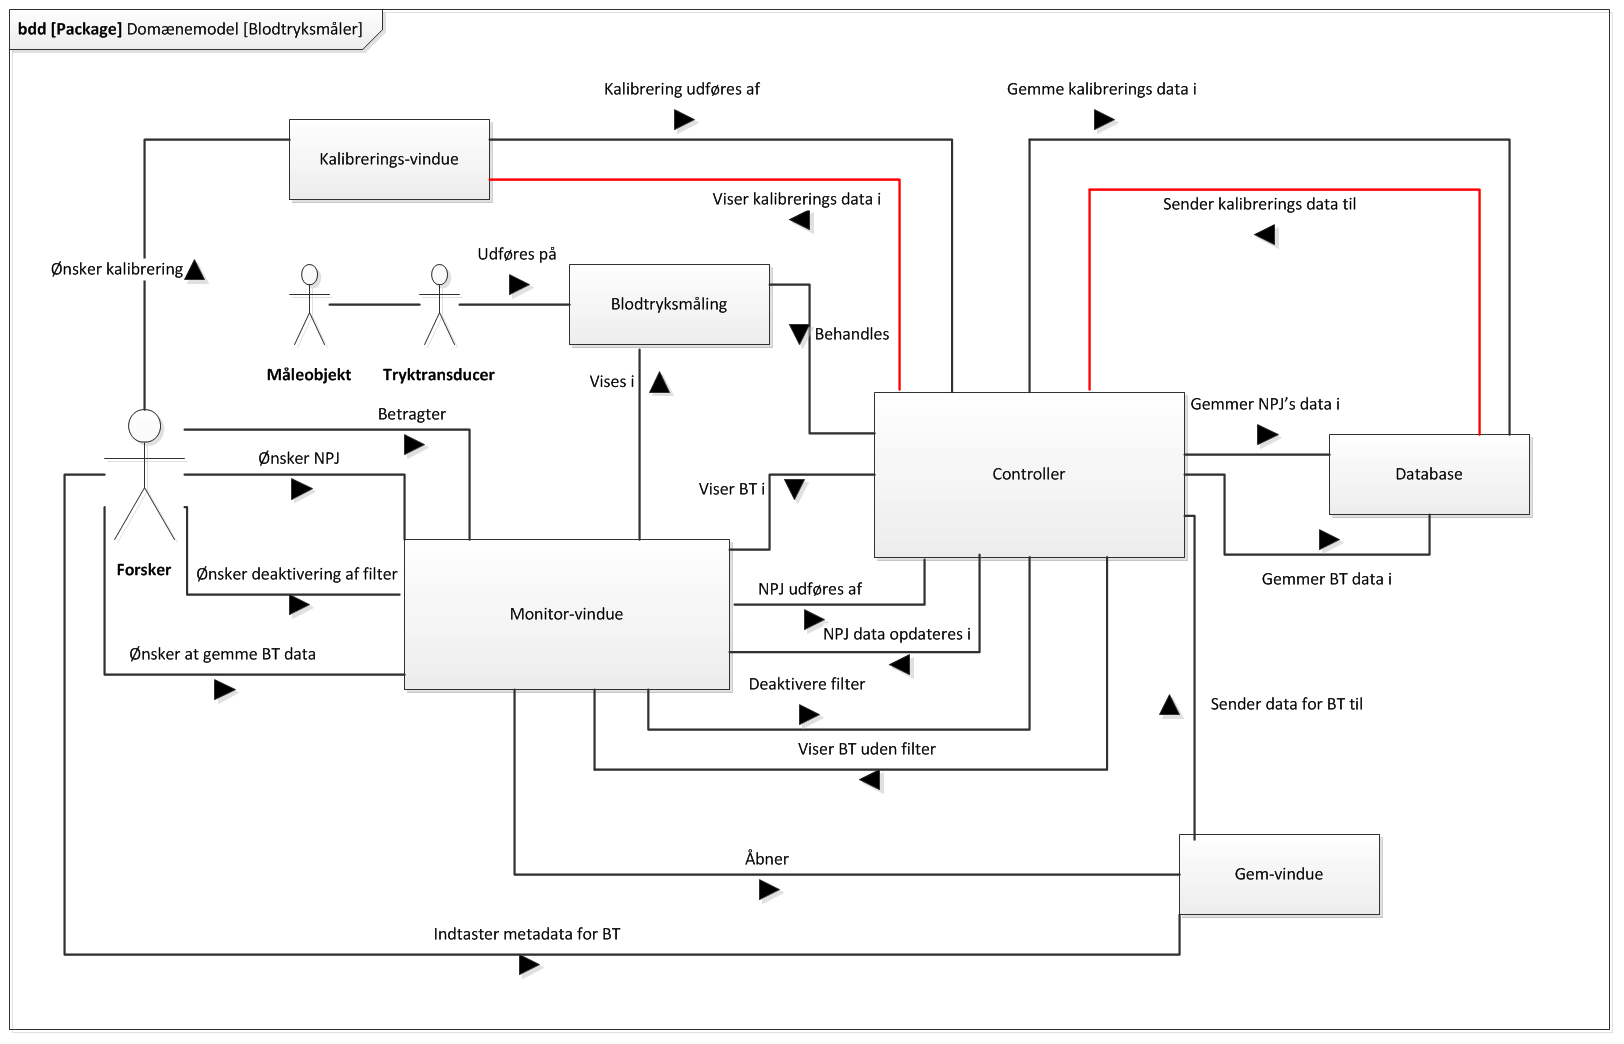
\includegraphics[width=1 \textwidth]{Figurer/Snip20151104_30}
	\caption{Domænemodel for blodtryksmålersystemet}
\end{figure}

NPJ = nulpunktsjustering\\
BT = blodtryksmåling
\\ \\
I domænemodellen ses to røde streger, som har hver deres kommando – ”kalibrerings data bliver sendt fra database” og ”vises i kalibrerings-vinduet”.Årsagen til at stregerne er røde, er, at hver af de to handlinger udelukkende forekommer ved start/genstart af programmet.

\subsection{Applikationsmodel}

\subsubsection{Sekvensdiagram}
Sekvensdiagrammerne beskriver step-by-step, via metoder, forløbet i de forskellige Use Cases. Der er lavet et sekvensdiagram for hver Use Case, for at gøre systemet mere overskueligt. Et sekvensdiagram består af boundary-klasserne og domain-klasserne fra domænemodellen, samt en controller-klasse, med navn efter den specifikke Use Case.

\begin{figure}[H]
	\centering
	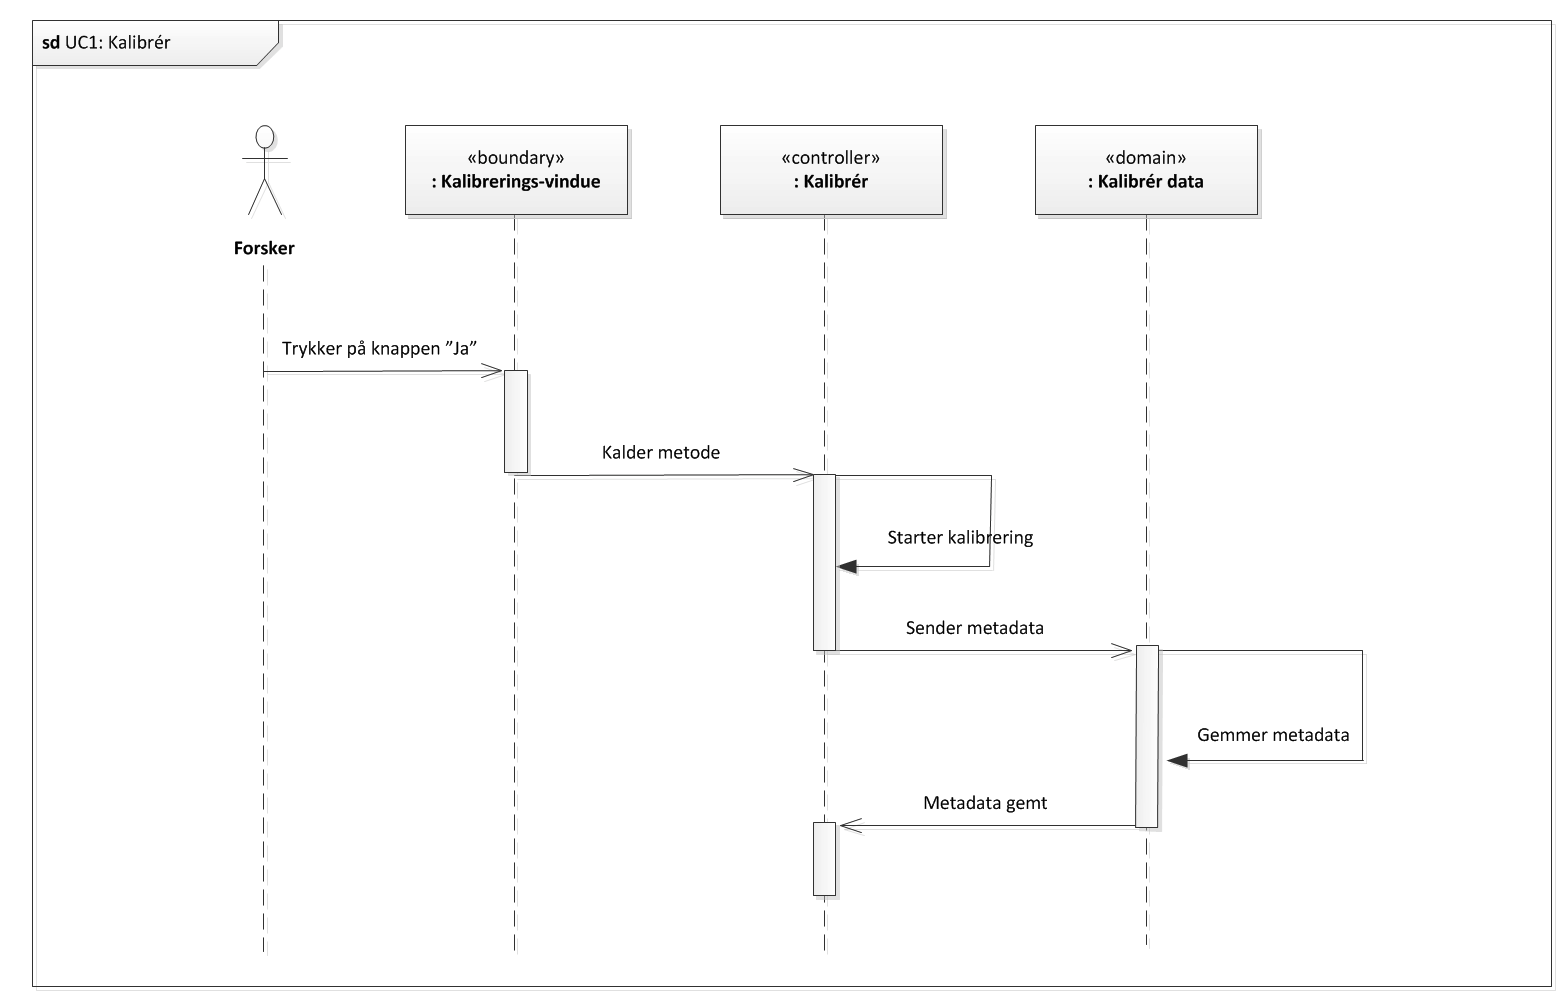
\includegraphics[width=1\textwidth]{Figurer/Snip20151104_31}
	\caption{Sekvensdiagram for UC1}
\end{figure}

Forsker interagerer med Monitorvindue. Kalibreringsmetoden bliver kaldt, når Forsker trykker på knappen ”Ja”. Derefter igangsættes kalibreringen og metadata sendes og gemmes. 

\begin{figure}[H]
	\centering
	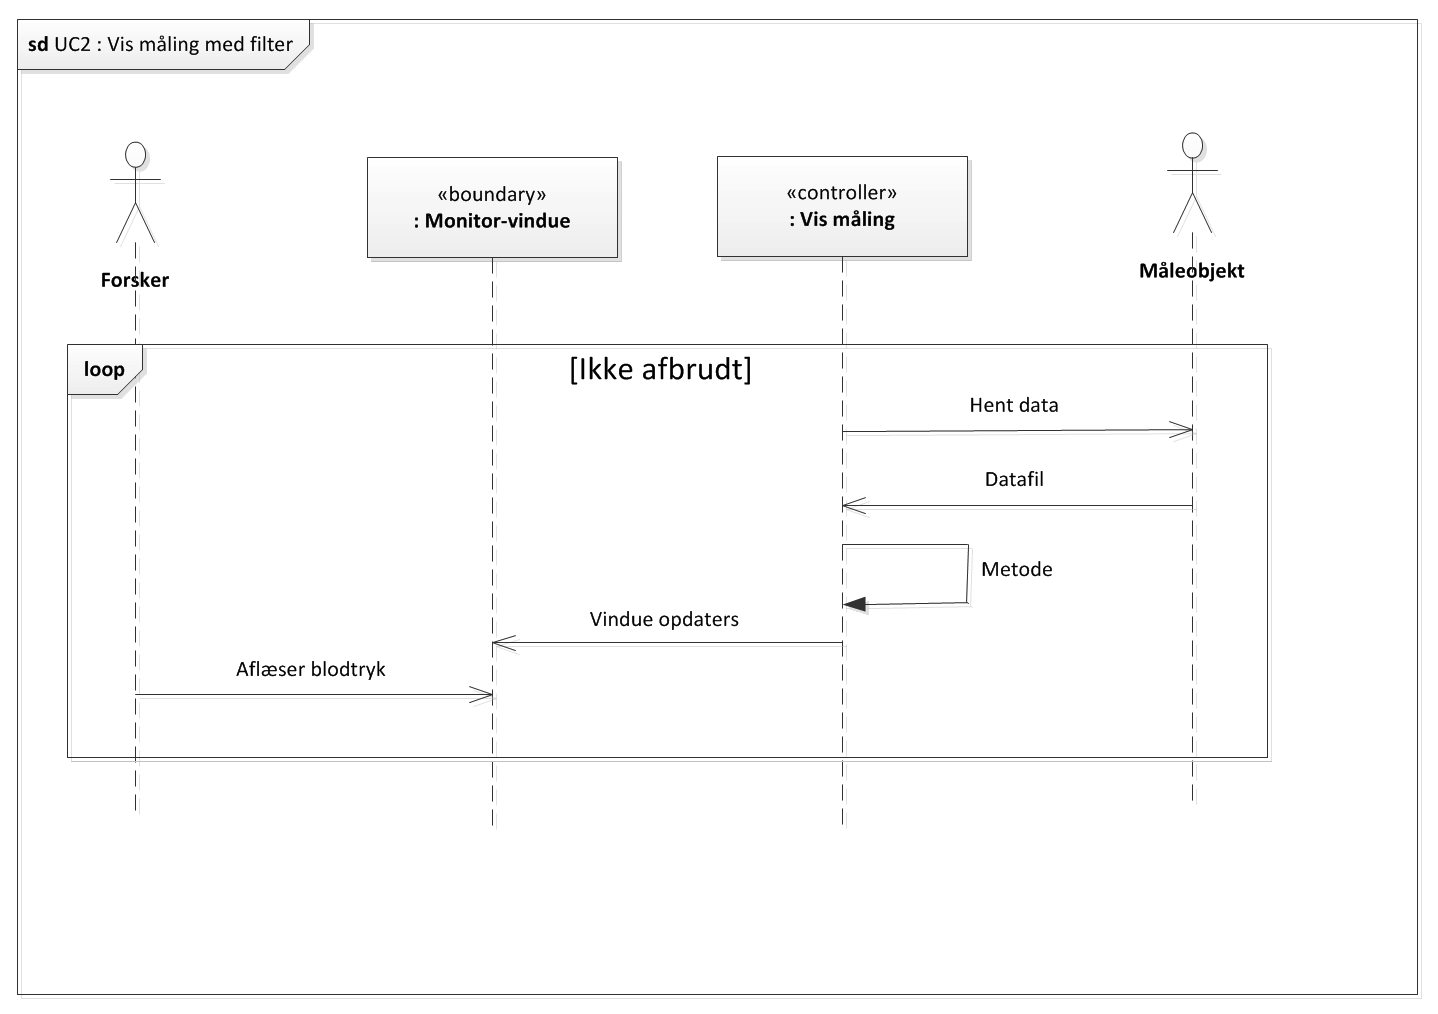
\includegraphics[width=1\textwidth]{Figurer/Snip20151104_32}
	\caption{Sekvensdiagram for UC2}
\end{figure}

Controller henter data fra Tryktransducer, som henter data i form af tryk fra måleobjekt. Datafilerne sendes fra Måleobjekt via Tryktransducer tilbage til Controller, der kalder metoden. Monitorvindue opdateres, og herefter kan Forsker aflæse blodtryk. 

\begin{figure}[H]
	\centering
	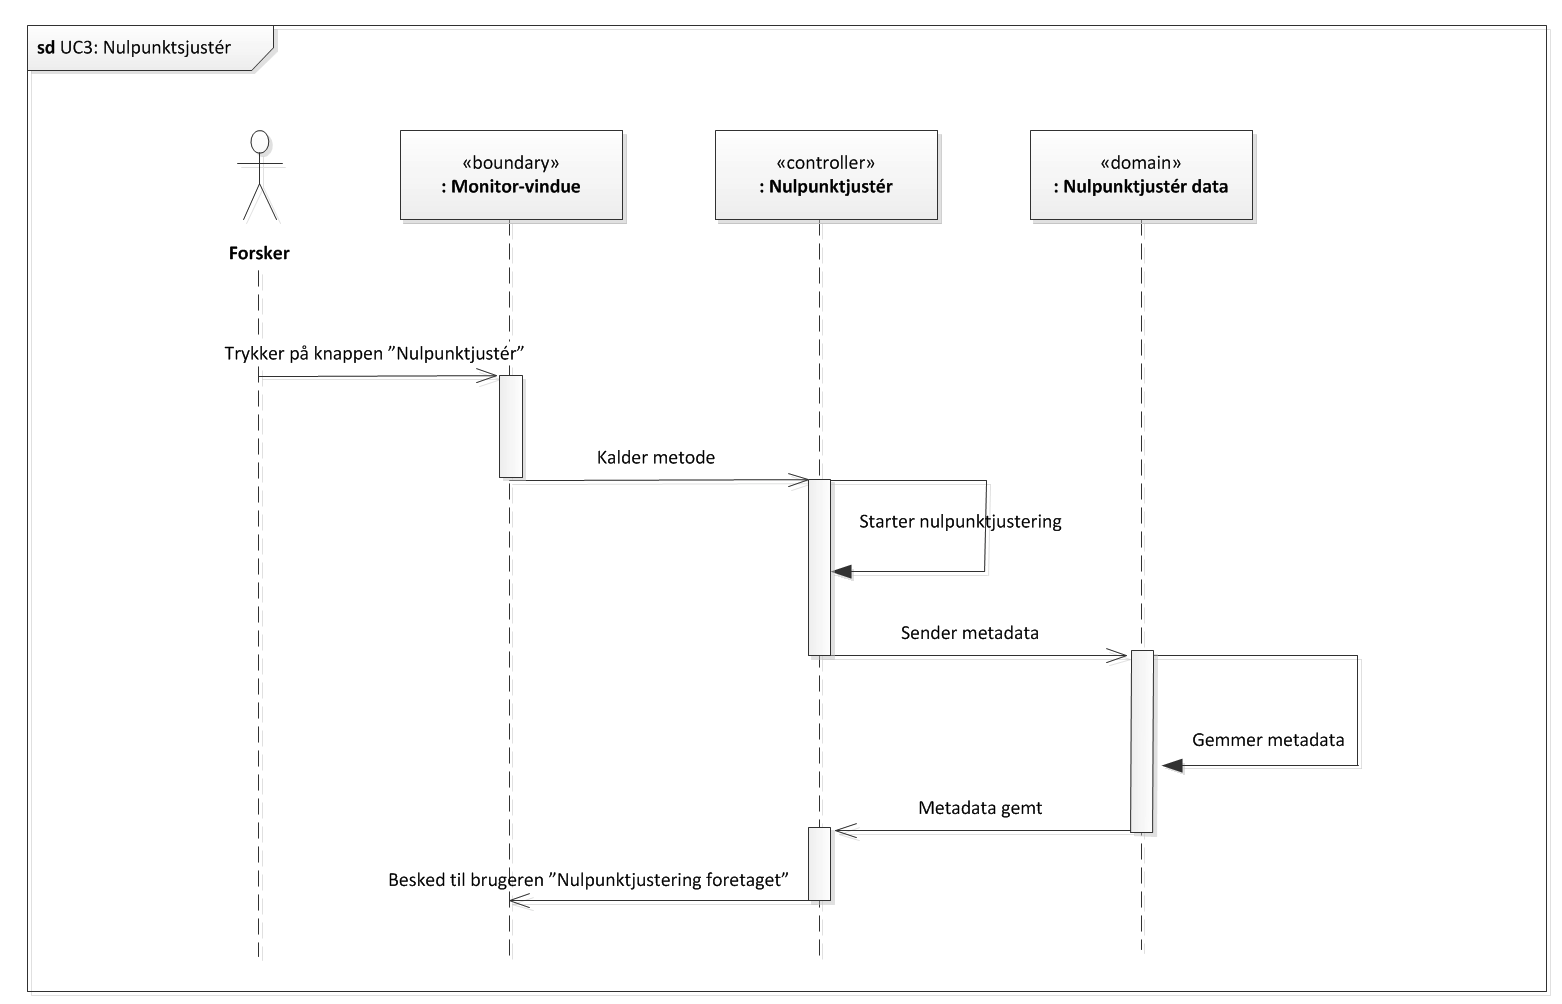
\includegraphics[width=1\textwidth]{Figurer/Snip20151104_33}
	\caption{Sekvensdiagram for UC3}
\end{figure}

Forsker interagerer med Monitorvindue ved at trykke på knappen ”Nulpunktsjustér”. Derefter kaldes metoden, og nulpunktsjusteringen startes. Metadata sendes og gemmes, hvorefter Forsker får besked om, at nulpunktsjusteringen er foretaget. 

\begin{figure}[H]
	\centering
	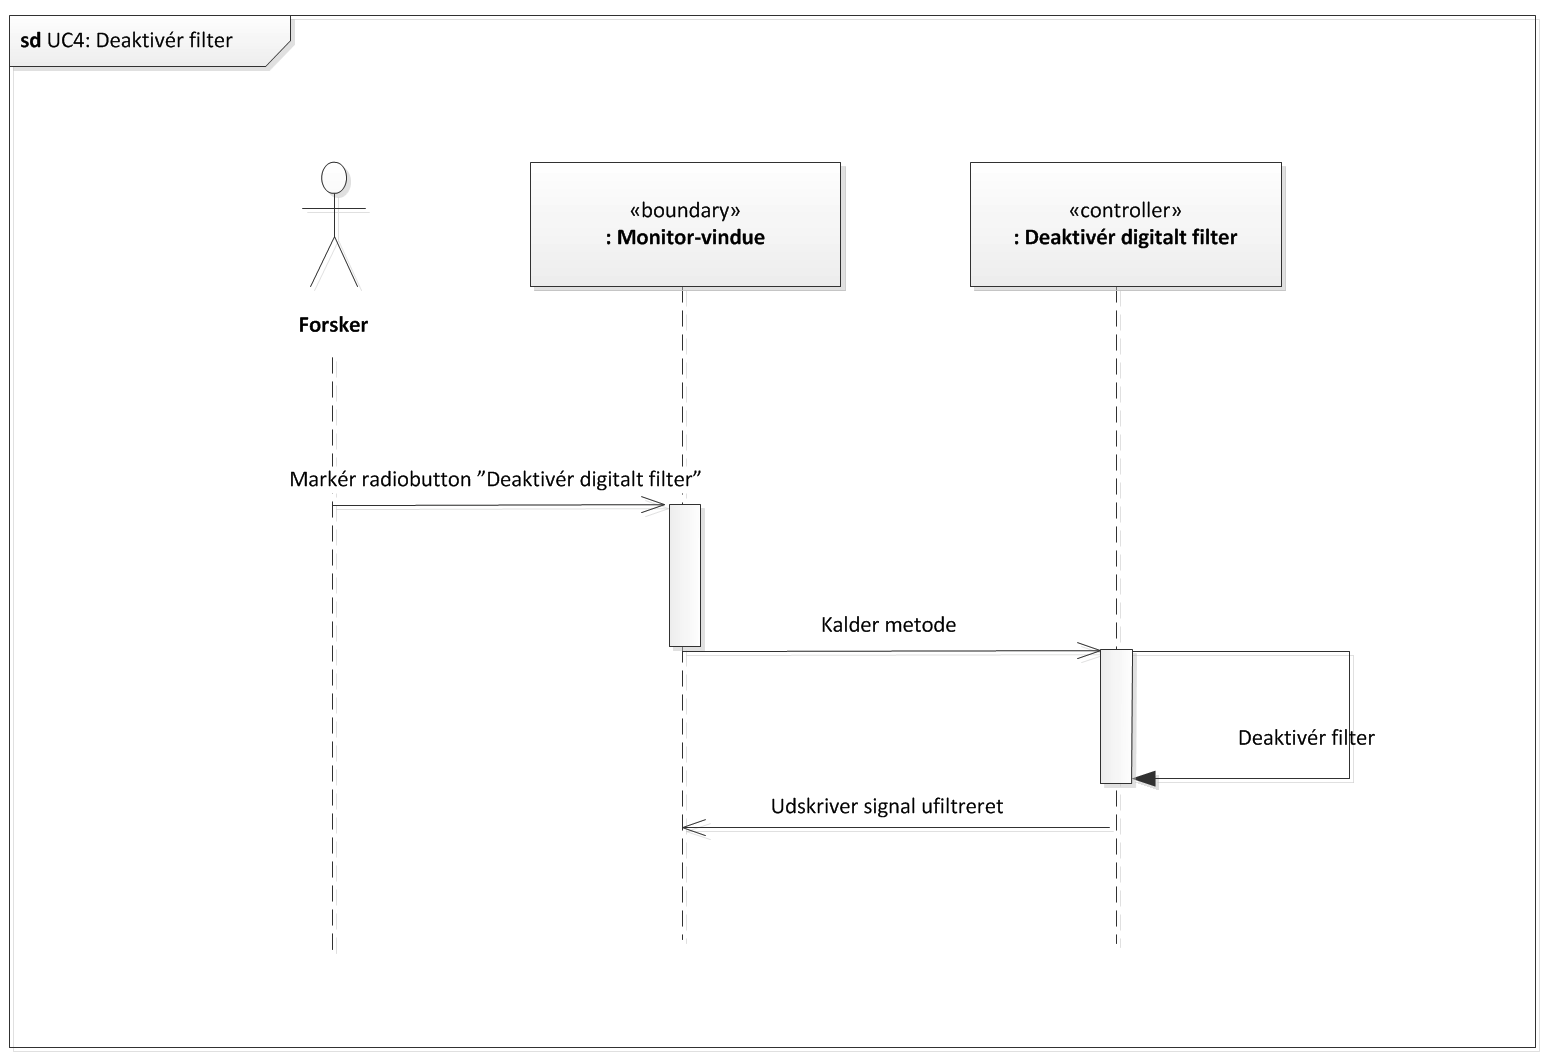
\includegraphics[width=1\textwidth]{Figurer/Snip20151104_34}
	\caption{Sekvensdiagram for UC4}
\end{figure}

Forsker interagerer med Monitorvindue ved at markere radiobutton ”Deaktivér digitalt filter”. Derefter kaldes metoden, og filteret deaktiveres, hvorefter signalet bliver udskrevet ufiltreret.

\begin{figure}[H]
	\centering
	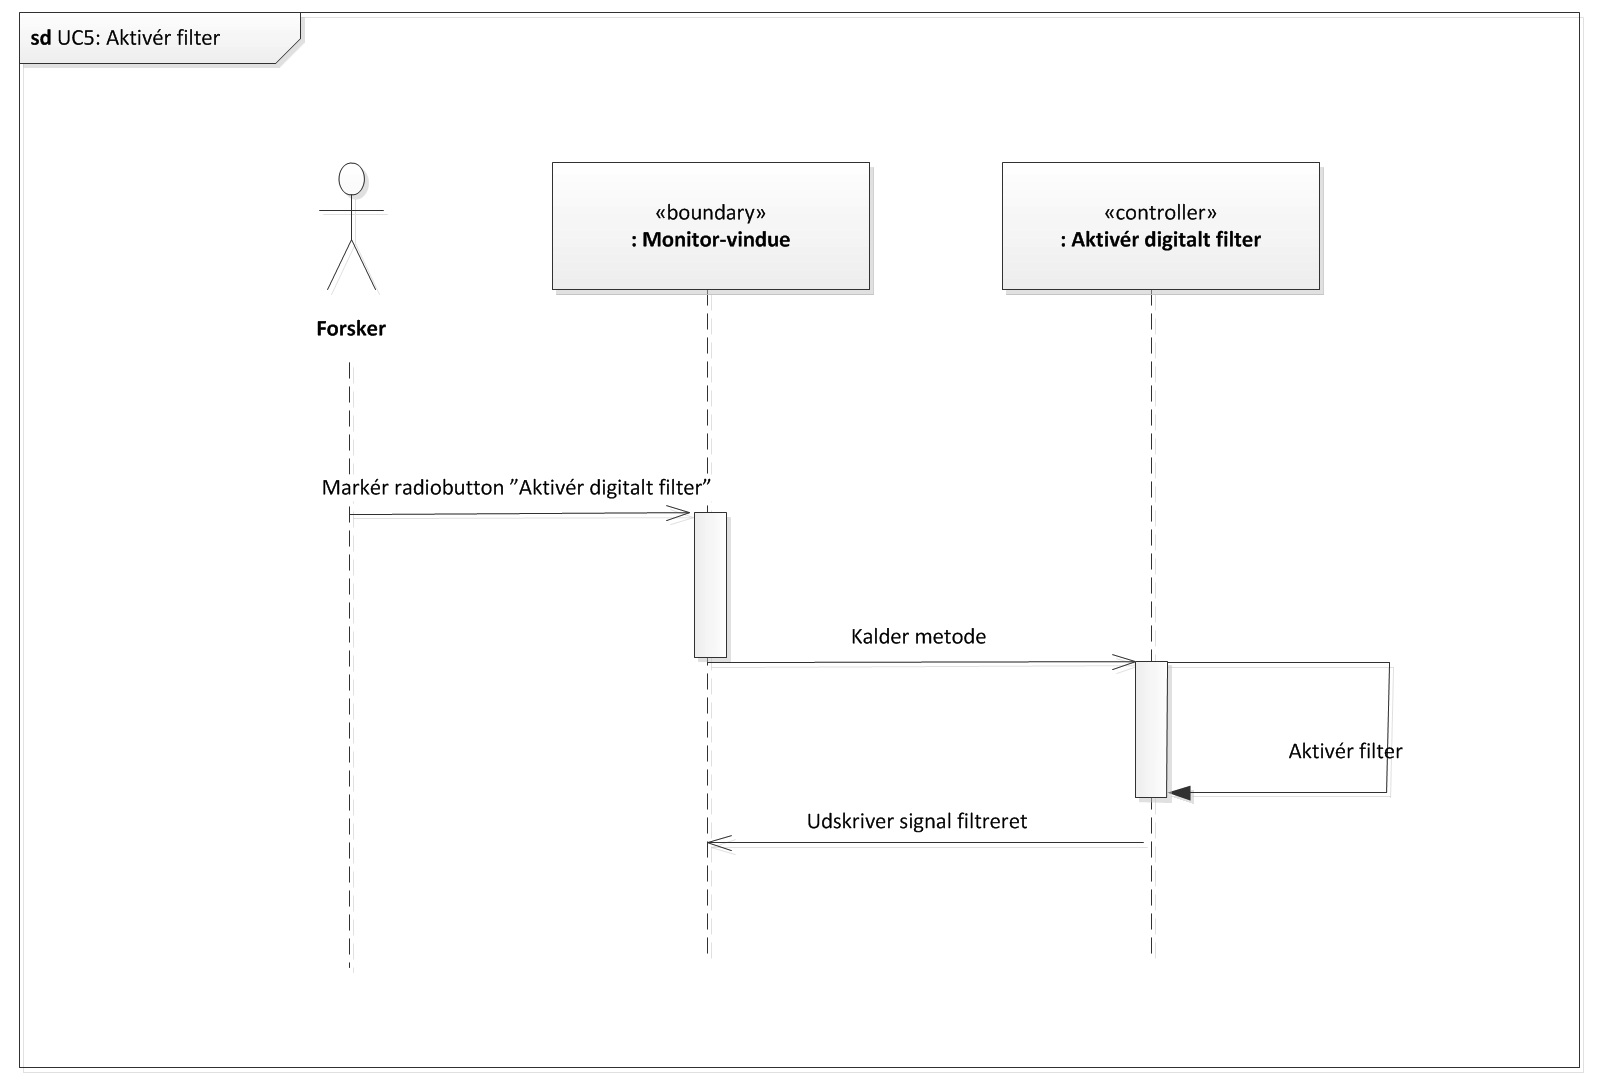
\includegraphics[width=1\textwidth]{Figurer/Snip20151104_35}
	\caption{Sekvensdiagram for UC5}
\end{figure}

Forsker interagerer med Monitorvindue ved at markere radiobutton ”Aktivér digitalt filter”. Derefter kaldes metoden, og filteret aktiveres, hvorefter signalet bliver udskrevet filtreret.

\begin{figure}[H]
	\centering
	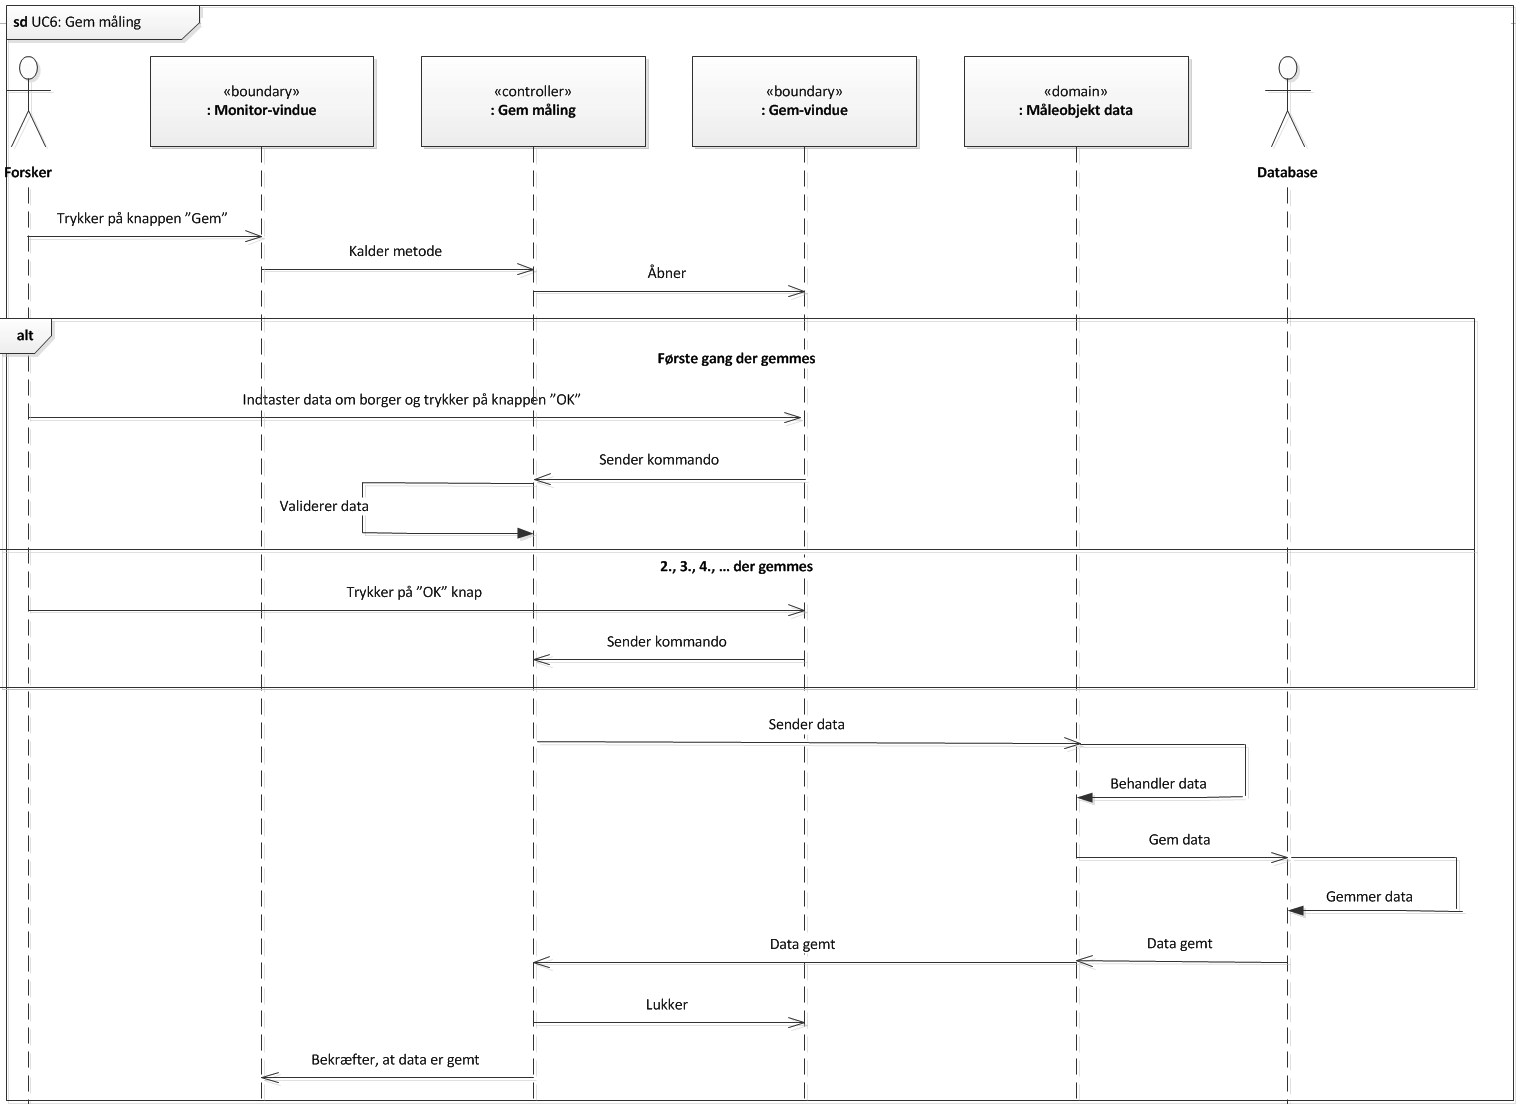
\includegraphics[width=1\textwidth]{Figurer/Snip20151104_36}
	\caption{Sekvensdiagram for UC6}
\end{figure}

Forsker interagerer med Monitorvindue ved at trykke på knappen ”Gem”. Derefter kaldes metoden og Gem vinduet åbnes. Første gang Forsker ønsker at gemme, indtastes data og der trykkes på knappen ”OK”. Kommando sendes og data valideres. De efterfølgende gange, der ønskes at gemme, er data udfyldt fra første gang, og der trykkes blot på ”OK”, hvorefter kommandoen sendes. Data sendes til datalag, hvor det bliver behandlet, og derefter bliver sendt til database. Data gemmes og Gem vinduet lukkes. Controller bekræfter til Monitorvindue, at data er gemt.

\subsubsection{Opdateret klassediagram}
De opdateret klassediagrammer indeholder metoderne fra de dertilhørende  sekvensdiagrammer - dette giver et overblik over, hvilke metoder de forskellige klasser består af.

\begin{figure}[H]
	\centering
	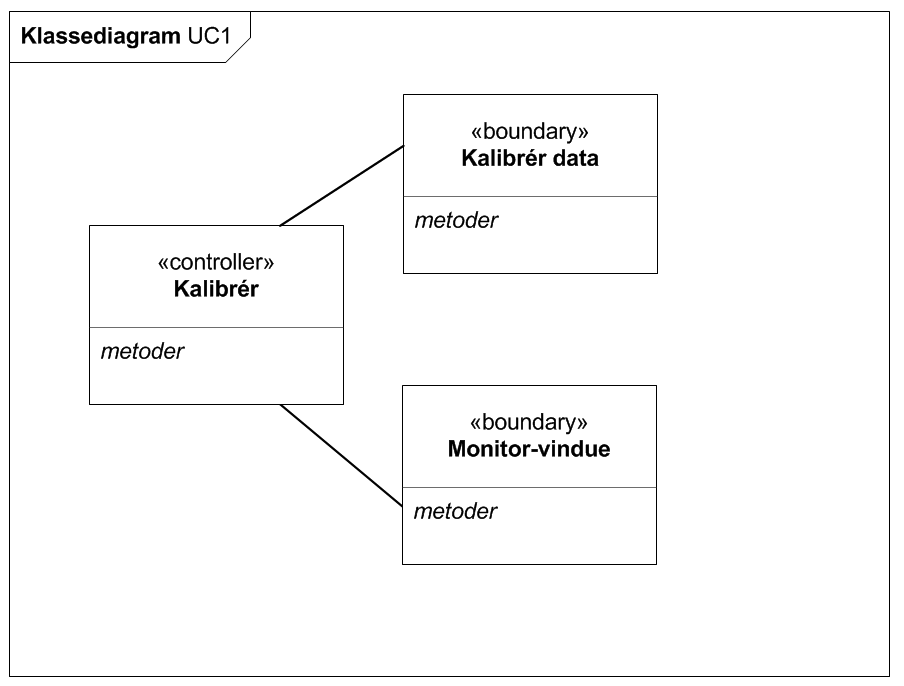
\includegraphics[width=1\textwidth]{Figurer/Snip20151104_37}
	\caption{Klassediagram for UC1}
\end{figure}
 

\begin{figure}[H]
	\centering
	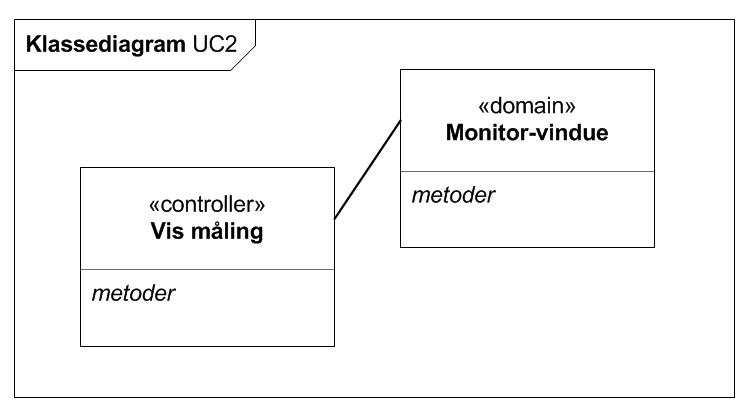
\includegraphics[width=1\textwidth]{Figurer/Snip20151104_38}
	\caption{Klassediagram for UC2}
\end{figure}

\begin{figure}[H]
	\centering
	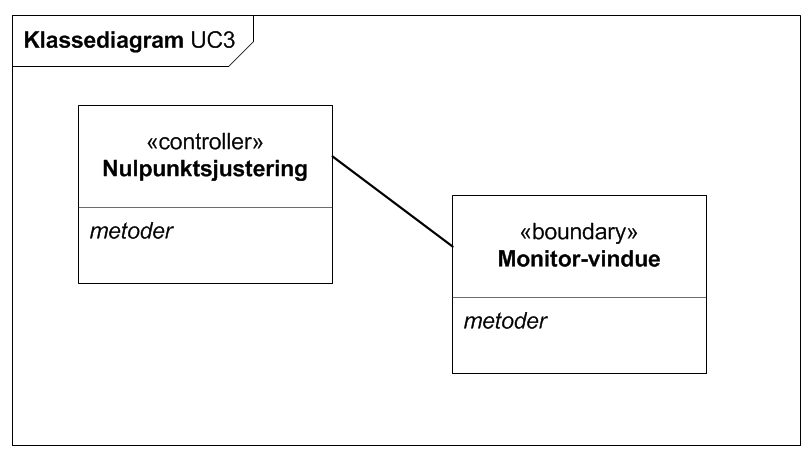
\includegraphics[width=1\textwidth]{Figurer/Snip20151104_39}
	\caption{Klassediagram for UC3}
\end{figure}

\begin{figure}[H]
	\centering
	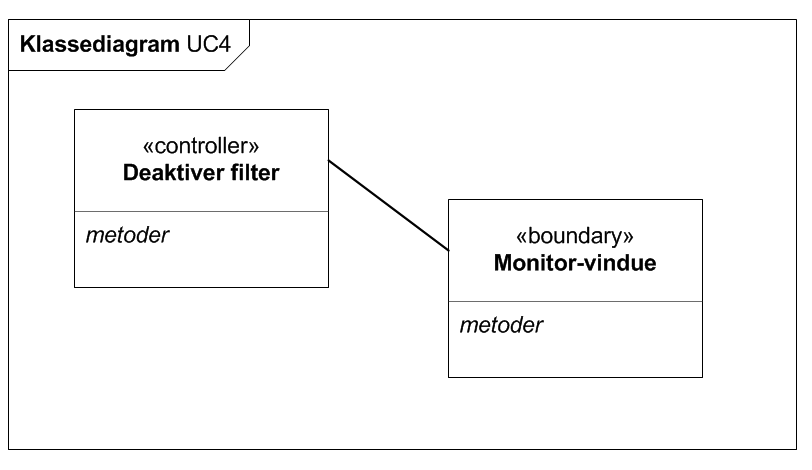
\includegraphics[width=1\textwidth]{Figurer/Snip20151104_40}
	\caption{Klassediagram for UC4}
\end{figure}

\begin{figure}[H]
	\centering
	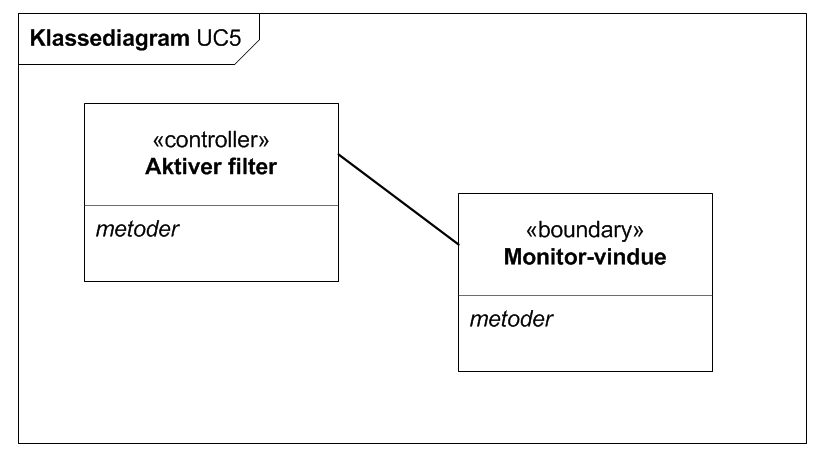
\includegraphics{Figurer/Snip20151104_41}
	\caption{Klassediagram for UC5}
\end{figure}

\begin{figure}[H]
	\centering
	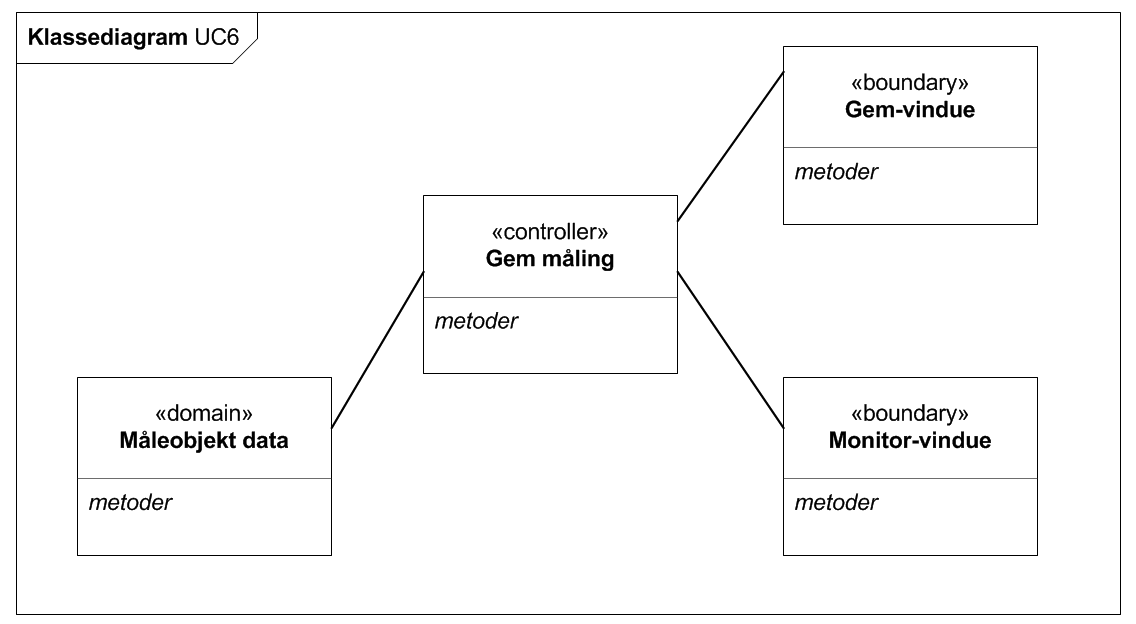
\includegraphics{Figurer/Snip20151104_42}
	\caption{Klassediagram for UC6}
\end{figure}












